\part{How can sounds be represent digitally?}
\frame{\partpage}

\begin{frame}{How Can Sound Be Represented Digitally?}
	\begin{itemize}
		\pause\item One method is to represent the wave itself and one
		approach to do this is \textbf{L}inear \textbf{P}ulse Code \textbf{M}odulation (LPCM).
		\begin{itemize}
			\pause\item An array of integers is created
			\pause\item The value of these integers represents the amplitude of the wave
			\begin{itemize}
				\pause\item  With linear coding, the way how bytes correspond to real-world
				measures - called \textit{quantisation} - is uniform across the range

			\end{itemize}
			\pause\item The positions in the array represent time, and so each element
			contains a sample of the wave amplitude 
		\end{itemize}
	\end{itemize}
\end{frame}

\begin{frame}{How Can Sound Be Represented Digitally? }
	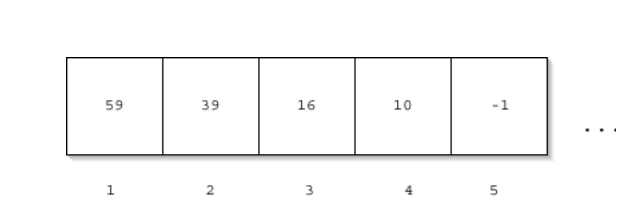
\includegraphics[width=\linewidth,height=0.7\textheight,keepaspectratio]{pcm_array}
\end{frame}

\begin{frame}{How Can Sound Be Represented Digitally?}
	\begin{itemize}
		\pause\item\textbf{Sample Rate:} How many samples are taken per second (consequently,
		how much time is represented by each element in the
		array)?

		\pause\item\textbf{Bit Depth:} How many bits are available to represent the value?
	\end{itemize}
\end{frame}

\begin{frame}{How Can Sound Be Represented Digitally?}
	\begin{itemize}
		\pause\item\textbf{Sample Rate:} i.e., range of frequencies which can be recorded
		array)?

		\pause\item\textbf{Bit Depth:} i.e., the number of amplitude levels which can be
		represented 
	\end{itemize}
\end{frame}

\begin{frame}{How Can Sound Be Represented Digitally? }
	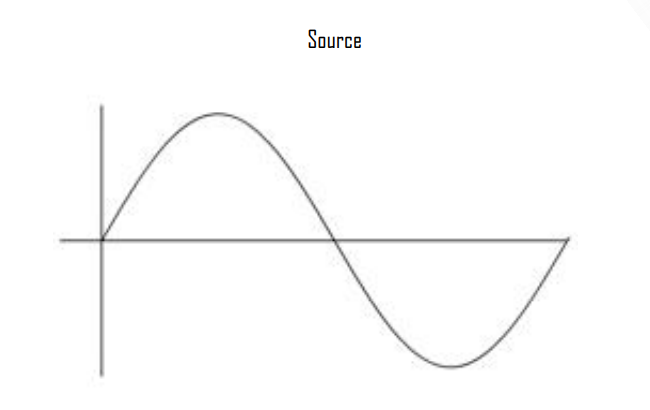
\includegraphics[width=\linewidth,height=0.7\textheight,keepaspectratio]{source_wave}
\end{frame}

\begin{frame}{How Can Sound Be Represented Digitally? }
	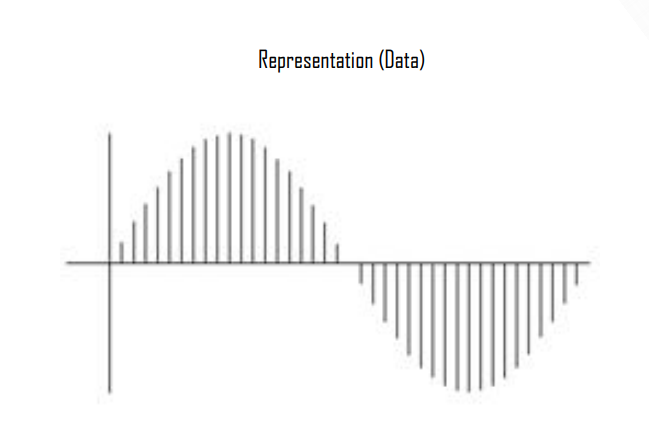
\includegraphics[width=\linewidth,height=0.7\textheight,keepaspectratio]{wave_data}
\end{frame}

\begin{frame}{How Can Sound Be Represented Digitally? }
	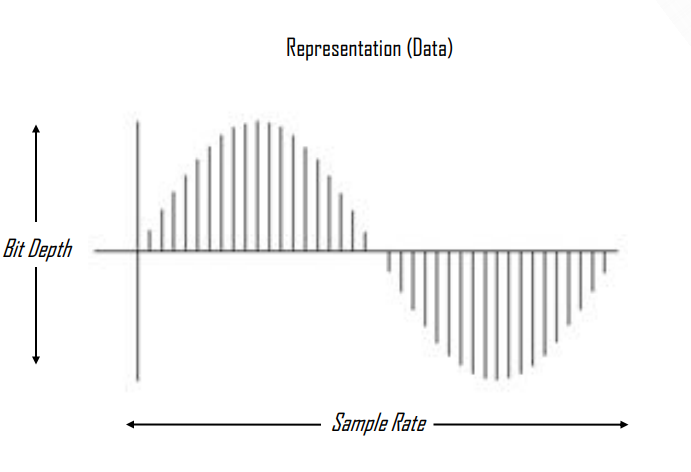
\includegraphics[width=\linewidth,height=0.7\textheight,keepaspectratio]{wave_axis}
\end{frame}

\begin{frame}{How Can Sound Be Represented Digitally? }
	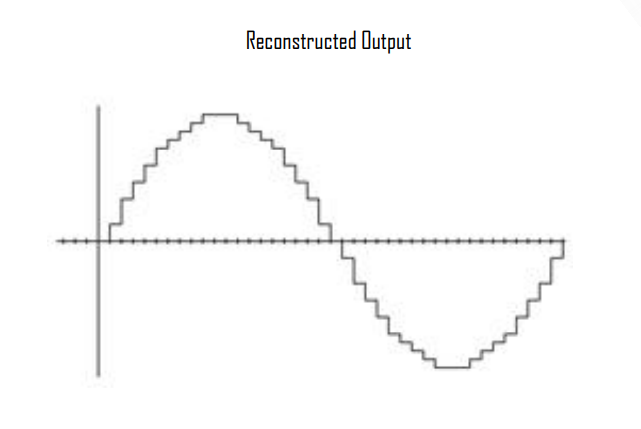
\includegraphics[width=\linewidth,height=0.7\textheight,keepaspectratio]{wave_reconstructed}
\end{frame}